\documentclass[tikz,border=10pt]{standalone}
\usepackage{amsmath}
\begin{document}
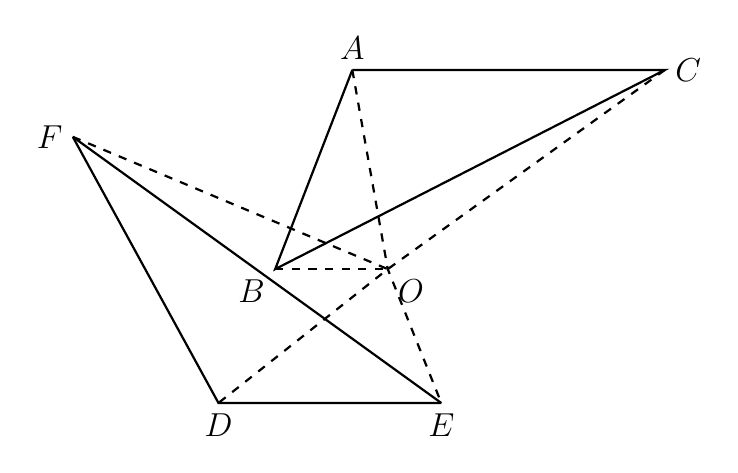
\begin{tikzpicture}[line width=0.8pt, font=\large]
  \coordinate (A) at (4.60,5.18);
  \coordinate (C) at (8.57,5.18);
  \coordinate (B) at (3.62,2.65);
  \coordinate (O) at (5.05,2.65);
  \coordinate (F) at (1.05,4.33);
  \coordinate (D) at (2.90,0.95);
  \coordinate (E) at (5.73,0.95);

  % solid edges
  \draw (A)--(B)--(C)--(A);
  \draw (F)--(D)--(E);
  \draw (F)--(E);

  % dashed edges
  \draw[dashed] (F)--(O);
  \draw[dashed] (B)--(O);
  \draw[dashed] (A)--(O)--(E);
  \draw[dashed] (C)--(O)--(D);

  % labels
  \node[above] at (A) {$A$};
  \node[right] at (C) {$C$};
  \node[left] at (F) {$F$};
  \node[below left] at (B) {$B$};
  \node[below right] at (O) {$O$};
  \node[below] at (D) {$D$};
  \node[below] at (E) {$E$};
\end{tikzpicture}
\end{document}
